\documentclass[twocolumn]{aastex62}

\usepackage[all]{nowidow}
\usepackage{stix}
\usepackage{xspace}
\usepackage{hyperref}
\usepackage{todonotes}
\usepackage{graphicx}

\newcommand{\vdag}{(v)^\dagger}
\newcommand\aastex{AAS\TeX}
\newcommand\latex{La\TeX}
\newcommand{\mjup}{\ensuremath{M_\mathrm{Jup}}\xspace}
\newcommand{\teff}{\ensuremath{T_{\mathrm{eff}}}\xspace}
\newcommand{\logg}{\ensuremath{\log(g)}\xspace}
\newcommand{\fluxunit}{\ensuremath{\mathrm{ergs}\,\mathrm{cm^{-2}}\,\mathrm{s^{-1}}\,\mathrm{\micron^{{-1}}}}}
\graphicspath{{./}{figures/}}
\shorttitle{HD106906b Time-Resolved Observations}
\shortauthors{Zhou et al.}
\newcommand{\editHL}[1]{{\color{blue}#1}}
\begin{document}


\title{Cloud Atlas: High-precision HST/WFC3/IR Time-Resolved Observations of Directly-Imaged Exoplanet HD106906b}

\correspondingauthor{Yifan Zhou}
\email{yzhou@as.arizona.edu}

\author{Yifan Zhou}
\affil{Steward Observatory}

\author{D\'aniel Apai}
\affil{Steward Observatory}

\begin{abstract}
 HD106906b is a $\sim11\mjup$ directly-imaged exoplanet orbiting at an extremely large distance from its host star. The wide separation between HD106906b and its host star greatly reduces the difficulty in direct-imaging observations, making it one of the most favorable directly-imaged exoplanets for detailed characterization. In this paper, we present results from HST/WFC3/IR time-resolved observations of HD106906b in the F127M, F139M, and F153M bands. We achieve 1\% precision in the lightcurves in all three bands. The F127M lightcurve demonstrates marginally-detectable variability with a best-fitting period of 4.02 hr, but the lightcurves in the other two bands are consistent with flat lines. We construct primary-subtracted deep images and use these images to exclude additional companions to HD106906 that are more massive than 2\mjup{} and locate at projected distances for more than $500$ au. We measure the astrometry of HD106906b in two HST/WFC3 epochs and achieve precisions better than 2.5 mas. The position angle and separation measurements are consistent with those in the 2004 HST/ACS images within 1$\sigma$. We provide the HST/WFC3 astrometric results for all visible background stars that can be used as reference sources in future precision astrometry studies. Our observations also provide the first 1.4 \micron{} water band photometric measurement for HD106906b. Fitting HD106906b's spectral energy distribution to the BT Settl model shows that the model over-predicts the HD106906b's water absorption depth and the best-fitting value for \logg{} is inconsistent with previous low to intermediate surface gravity assessment. These inconsistencies highlight the challenges in modeling atmospheres of young planetary-mass objects.
\end{abstract}

\keywords{Planetary Systems --- planets and satellites: atmospheres --- methods: observational}

\section{Introduction}

Condensates clouds are central components of the atmospheres of brown dwarfs and exoplanets \citep[e.g.,][]{Morley2012,Marley2013,Marley2015}. Cloud opacity strongly impacts the near-infrared color and spectra of these objects. Therefore, understanding cloud properties is critical to determining  fundamental properties and atmospheric compositions of substellar objects through emission and transmission spectroscopic observations \citep{Ingraham2014, Kreidberg2014a, Stevenson2016, DeWit2016, Samland2017}. Because brown dwarfs are available for direct spectroscopy and their observations are generally less challenging than transmission spectroscopy of transiting exoplanets, cloud properties for brown dwarfs are better constrained than for exoplanets through time-averaged spectroscopic \citep[e.g.,][]{Cushing2008,Stephens2009} and {time-resolved} \citep[e.g.,][]{Buenzli2012,Apai2013,Biller2017,Apai2017} observations. Directly-imaged exoplanets and planetary-mass companions \citep[e.g.,][]{Chauvin2004,Marois2008a,Marois2010,Macintosh2015a}, which overlap with transiting planets in mass and are suitable for high-quality time-series observations, are excellent targets for connecting cloud studies between brown dwarfs and exoplanets.

HD106906b is an $11\pm2$ \mjup{}  mass exoplanet orbiting an F5V spectral-type star \citep{Bailey2013}. The HD106906 system, at a distance of $103.3\pm0.4$ pc \citep{Gaia2016,Gaia2018}, is a member of the Lower Centaurus Crux association (99.8\% membership probability based on BANYAN-$\Sigma$, \citealt{Gagne2018} ), which itself is  part of the Sco-Cen OB association \citep[age: $15\pm3$ Myr,][]{Pecaut2016}. The planet has a wide separation of $7\arcsec.11\pm0\arcsec.03$ from its host star \citep{Bailey2013}, corresponding to a projected distance of $734\pm4$ au. Because of its wide angular separation to its host and moderate brightness contrast ($\Delta J=10.3\,\mathrm{mag}$ at 10.3\arcsec), HD106906b is among the most favorable exoplanets for atmospheric characterizations \citep[e.g., ][]{Bailey2013,Kalas2015,Wu2016,Daemgen2017}

Multi-wavelength photometric \citep{Bailey2013,Kalas2015,Wu2016} and spectroscopic \citep{Bailey2013, Daemgen2017} observations have been used to characterize HD106906b's atmosphere.  These studies agree on an effective temperature (\teff) of 1800~K and a spectral type classification of L2.5-3. Based on its ``triangular-shaped'' $H$-band spectrum, both \citet{Bailey2013} and \citet{Daemgen2017} classified HD106906b as an intermediate to low surface gravity object. The low surface gravity classification is also consistent with its young age. Similar to many other young L-type planetary-mass objects (2M1207b, HR8799bcde, PSO J318), HD106906b has reddened near-infrared (NIR) colors compared to those of the field brown dwarfs of the same spectral type. The reddened NIR color is often associated with dusty atmospheres and thick condensate clouds \citep[e.g.,][]{Skemer2011}. Time-resolved observations of these reddened objects have often found  them to be variable \citep[e.g.,][]{Biller2015,Zhou2016,Lew2016,Vos2017,Biller2017,Manjavacas2017,Zhou2019}. The most convincing explanation for their variability is heterogeneous clouds rotationally modulating the integrated flux from HD106906b's photosphere. Consequently, multi-wavelength NIR rotational modulation became an effective tool to study condensate clouds, particular vertical cloud profiles for brown dwarfs and planetary mass objects \citep[e.g.,][]{Apai2013, Biller2017, Zhou2018}. Therefore, it is likely that high-precision time-resolved NIR observations will also be an effective method to explore the cloud properties of HD106906.

HD106906b's extremely wide orbit and its deviation from the host star's circumstellar plane pose challenges in explaining its formation. Disk fragmentation has difficulty forming a planet/companion with a mass as small as that of HD106906b \citep[e.g.,][]{Kratter2010}. High-contrast direct-imaging survey results strongly support core accretion as the formation pathway of planetary-mass companions with orbits smaller than 100~au \citep{Wagner2019,Nielsen2019}.  At a projected distance of more than 700~au from its host star, it is unlikely for HD106906b to accrete enough material through \emph{in situ} core accretion. A $\sim21^{\circ}$ projected angle between the planet's position angle and the plane of its host star's disk \citep{Kalas2015} further argues against \emph{in situ} core accretion but suggests dynamical orbit evolution of this planet \citep[e.g.,][]{Marleau2019}.  \citet{DeRosa2019} discovered a close, near-coplanar stellar encounter with the HD106906 system, further supporting a conjecture of intense dynamical activity in the system's evolution history. Considering these evidence suggesting past dynamical evolution, it should not be surprising if HD106906b has an eccentric orbit. Therefore, astrometric constraints on the orbit of HD106906b will be critical for understanding the formation and evolution history of HD106906b.

In this paper, we analyze and discuss \emph{Hubble Space Telescope} Wide Field Camera 3 near-infrared channel (HST/WFC3/IR) observations of HD106906b in time-resolved direct-imaging mode. We present light curves of HD106906b in three bands that cover the 1.4\micron{} water band and its the continuum. We look for variability in the light curves and use them to discuss the atmospheric and cloud properties of HD106906b. We also compare the relative astrometry of HD106906 system in the two WFC3 observations and in the HST Advanced Camera for Survey/High-Resolution Channel (ACS/HRC) observations, which were taken in 2004. The WFC3 and ACS/HRC observations together form a high astrometric precision  image series with 14 years baseline,  which can place tight constraints on the relative motion of HD106906b relative to its host star.

\section{Observations}
The HST/WFC3/IR observations of HD106906 are part of the HST Large Treasury program \emph{Cloud Atlas} (Program ID: 14241, PI: D. Apai). We observed HD106906 from 2016-01-29 20:45 to 2016-01-29 23:02 UTC for two consecutive HST orbits as part of the program's variability amplitude assessment survey (VAAS). We then used the same instrument set-ups to re-visit the target from 2018-06-07 02:14 to 2018-06-07 12:35 UTC  for seven consecutive HST orbits as part of the deep look observations (DLO). Dithering was not applied during the observation to reduce systematics caused by flat field errors. The target was observed in F127M ($\lambda_{\mathrm{pivot}}=1.274\micron$, $\mathrm{FWHM}=0.07\micron$), F139M ($\lambda_{\mathrm{pivot}}=1.384\micron$, $\mathrm{FWHM}=0.07\micron$) and F153M ($\lambda_{\mathrm{pivot}}=1.533\micron$, $\mathrm{FWHM}=0.07\micron$) filters.  The filter selection allows comparison of the modulations  in (F139M) and out  (F127M, F153M) of the 1.4 \micron{} water absorption band.  Exposure times were 66.4 seconds for the F127M and F153M observations and 88.4 seconds for the F139M observations. We alternated these three filters in every two or three exposures, and thus the light curves in the three filters are \emph{de facto} {contemporaneous}. 

The observations are designed to enable two-roll angular differential imaging for primary point spread function (PSF) star subtraction.  This technique was successfuly applied in HST high-contrast observations \citep[e.g.,]{Zhou2016,Zhou2019}. {Successive orbits alternately differed in celestial orientation angle 31 degrees apart, with odd (1, 3, 5, and 7), and even (2, 4, 6) numbered orbits respectively at the same orientations.} Subtracting images  taken in the odd orbits from those  taken in the even orbits (or vice versa) removes the primary star PSF (in the absence of systemmatics to the level of the photon noise) but conserves the companion PSF (Figure \ref{fig:2rdi}).  

HD106906 was also observed by HST/ACS/HRC on 2004-12-01 UTC (PID: 10330, PI: H. Ford). The 2004 ACS/HRC observations include two identical 1,250 seconds direct-imaging exposures in the ACS F606W  band. We use results  from these observations \citep{Bailey2013,Kalas2015} to extend the temporal baseline for our astrometric analysis.

\section{Data Reduction}
% \subsection{Time-resolved photometry}

\subsection{Time-Resolved Photometry}
\begin{figure*}
  \centering
\plottwo{figures/F153M_medianSubtractionMasked_rotation_01}{figures/HD106906_RGB_composite}  
  \caption{Direct-imaging observations of the HD106906 system. \emph{Left:} An illustration for the 2RDI results. Red color represents signals from the original images and blue colored pixels are structures from the subtraction model images. Regions that are marked by hatches are used for optimizing the subtraction. \emph{Right: An R (F153M) G (F139M) B (F127M) color composite image of HD106906.} Overlaid on the HST RGB composite are the false-color GPI (inner most) and ACS/HRC (outer annulus) scattered light images \citep{Kalas2015} of the circumstellar disk. The circumstellar disk is not visible in the WFC3/IR images.}
  \label{fig:2rdi}
\end{figure*}

Time-resolved photometry for HD106906b starts with \texttt{flt} files produced by the CALWFC3 pipeline. Our photometric data reduction has four steps: data preparation, primary star subtraction, PSF fitting photometry, and light curve systematics removal. Reductions for light curves in the three filters are independent. Therefore, the four reduction steps are applied to observations in three filters in parallel. 

In the data preparation step, we sort \texttt{flt} images into data cubes. We first build bad pixel masks and remove the sky background. Pixels that have data quality flags 4 (bad detector pixel), 16 (hot pixel), 32 (unstable response), and 256 (full-well saturation) are identified as ``bad pixels'', masked out, and excluded from subsequent analyses. After masking out pixels with data quality warning flags, we further examine images by eye to identify and mask out remaining spurious pixels. To remove the sky background, we first draw circular masks around all visible point sources in the field and then apply a five-iteration $5\mbox{-}\sigma$ sigma-clip to exclude remaining bright pixels that are not part of the sky background. We take the median value of the unmasked pixels as sky background and subtract it from every image. The background-subtracted images and the associated bad pixel masks are sorted in chronological order and stored in data cubes.

We then apply two-roll differential imaging (2RDI) to subtract the PSF of the primary star.  Images taken with the first telescope roll are subtraction template candidates for images taken with the second telescope roll and vice versa. We first register images by the centroid of the primary star using two-dimensional cross-correlation and align the images with bi-linear interpolation shift. We then  refine image registration by least $\chi^{2}$ optimization in regions affected by diffraction on the secondary mirror support structures. We then select the best subtraction template from all available candidate images.  Each subtraction template candidate is linearly scaled to minimize the squared summed subtraction residuals in the original$-$template image in an annulus around HD106906A (Figure \ref{fig:2rdi}). The best subtraction template is the one that results in the smallest subtraction residuals. Finally, we subtract the best templates from the original images to obtain primary subtracted images (Figure \ref{fig:2rdi}). 

HD106906b's flux intensity is measured by PSF fitting to the primary subtracted images. Details of the PSF fitting procedures can be found in \citet{Zhou2019}. We construct $9\times$ over-sampled PSFs using the TinyTim PSF modeling software \citep{Krist1995}. Free parameters for the model PSFs are the centroid coordinates, HST secondary mirror displacement, and the amplitude of the PSF. We optimize these parameters using a maximum likelihood method combined with Markov Chain Monte Carlo (MCMC) algorithms \citep[MCMC performed by \texttt{emcee},][]{Foreman-Mackey2012}. Aperture correction for each filter band is done through PSF fitting photometry as we normalize the model PSF to flux within an infinitely large aperture. 

The random noise of the light curves is composed of  photon noise, detector readout noise, and noise from dark current. Light curve analyses require systematic noise in the light curve to be accurately characterized and corrected. For WFC3/IR light curves, charge trapping related ramp effect is the major component of light curve systematic noise. We use RECTE \citep{Zhou2017} to model and remove the ramp effect systematics from the light curves. Our implementation of the ramp effect removal procedure follows \citet{Zhou2019}, in which details of the application of RECTE in time-resolved direct imaging observations are provided. We calculate ramp profiles by feeding the entire time series into RECTE and forward-modeling the charge trapping systematics. The model ramp profiles are divided from the light curves to correct the systematics. Figure~\ref{fig:lightcurve} shows the corrected light curves.

\subsection{Astrometry}
We follow the procedure detailed in \citet{Bedin2018} for astrometric measurement.
We first measure the raw Cartesian $(x, y)$ coordinates by fitting empirically derived PSFs to the \texttt{flt} images using a software that is adapted from the program \texttt{img2xym\_WFC.09x10}, which is initially developed for ACS/WFC \citep{Anderson2006} and extended for WFC3/IR \citep{Bedin2018}. The empirical PSFs are from publicly available PSF library released by STScI \footnote{\url{http://www.stsci.edu/~jayander/WFC3/WFC3IR\_PSFs/}}.  We then apply the most updated geometry correction for WFC3/IR  (derived by J. Anderson and is publicly available \footnote{\url{http://www.stsci.edu/~jayander/WFC3/}}) to obtain geometrically corrected positions. The corrected Cartesian coordinates within a same epochs are then sigma-clipped averaged,  safely assuming no (sizable) intrinsic motion of sources observed within a same given epoch. These procedures derive result in geometrically corrected Cartesian coordinates and their uncertainties for each source in each epoch.

We then transform the corrected Cartesian coordinates to the equatorial coordinate system (right ascension, {R.A.}, $\alpha$ and declination, {Dec.}, $\delta$). Common stars are used to find the most general linear transformation (six parameters) that converts $(x, y)$ to $(\xi,\eta)$ (equatorial $\alpha$ and $\delta$ coordinates' projections on the tangent plane) or vice versa. $(\xi, \eta)$ are then transformed to $(\alpha, \delta)$ using Equations (3) and (4) in \citet{Bedin2018}.
Considering the non-linearity in $(x, y)$ to $(\alpha, \delta)$ transformation, we adopt a Monte Carlo approach to derive the uncertainties in {R.A.} and {Dec.}  For every source, we generate 1,000 Gaussian distributed samples of $(x, y)$  based on the best-fitting values and their uncertainties. We then transform the Cartesian list  to  a list of {R.A.} and {Dec.} pairs. We calculate the standard deviations of the {R.A.} and {Dec.} as their $1$-$\sigma$ uncertainties. We note that the uncertainties in R.A. and Dec. include PSF-fitting uncertainties but not systematic uncertainties that can be introduced by motions of the reference sources that are used to establish the $(x, y)$ to $(\xi,\eta)$ transformation.

\section{Results}
% \subsection{Image}
\subsection{Photometry, Lightcurves, and Variability}

Figure~\ref{fig:lightcurve} shows the corrected and normalized lightcurves in the F127M, F139M, and F153M bands. For single image photometry, we achieve average SNRs of  77, 78, and 105 in the F127M, F139M, and F153M bands, respectively. The time-averaged absolute flux intensity\footnote{The conversions are done using the \texttt{PHOTFLAM} values listed in fits file headers.} in these three bands are $6.23\pm0.08\times10^{-13}\fluxunit$, $3.71\pm0.05\times10^{-13}\fluxunit$, and $4.35\pm0.04\times10^{{-13}}\fluxunit$, respectively.
%The flux uncertainties are for average $1-\sigma$ uncertainty in a single image.
For the light curves, variations with zero-to-peak amplitude $>1\%$ rotational modulations are not detected in any bands. We find that variations in the light curve are dominated by random noise for which the major component is the photon noise. Relative to flat lines, the three light curves have reduced-$\chi^{2}$ of 1.89, 1.47, and 1.1 in the F127M, F139M, and F153M bands, respectively.

We calculated the Lomb-Scargle power spectra \citep[][Figure~\ref{fig:periodogram}]{Lomb1976} of the lightcurves to investigate lightcurve periodicity. The power spectra for the F139M and F153M lightcurves do not show any significant peaks except in the high-frequency (short periodicity) region, where the power spectra are dominated by random noise. The lack of signals in the F139M and F153M power spectra is consistent with the featureless lightcurves. The power spectra for the F127M lightcurve has a peak at 4.02 hr. Compared to a flat line, the best-fitting single sine wave with period fixed at 4.02~hr marginally decreases the reduced-$\chi^{2}$ from 1.89 to 1.53. The best-fitting amplitude of the 4.02 hr sine wave is $A = 0.49\pm0.12\%$ with phase offset of $\Delta \phi = -1.57\pm0.29$ rad. Figure~\ref{fig:fold} shows the F127M lightcurve folded to the 4.02 hr period.

We use a bootstrap method \citep{Manjavacas2017,Zhou2019} to evaluate the significance of the periodogram signal, and show the result in Figure \ref{fig:periodogram}. This analysis yields a $2.66\sigma$ significance of the 4.02 hr periodic signal. The 4.02 hr periodic signal also overlaps with a side-lobe of the periodogram of the observation window functions. The low SNR and the effect from observation window function argue \emph{against} 4.02 hr signal being a robust detection of periodicity in the lightcurve.

In summary, HD106906b only shows marginal  evidence of variability in the F127M band. Lightcurves in the other two bands (water absorption, the red side of water band continuum) are consistent with flat lines.

\begin{figure}[!ht]
  \centering
  \plotone{figures/HD106906_lightcurves.pdf}
  \caption{HST/WFC3/IR Lightcurves for HD106906b in the F127M, F139M, and F153M bands. For clarity,  offsets of 5\% and 10\% are applied to the F139M and F153M lightcurves, respectively.}
  \label{fig:lightcurve}
\end{figure}

\begin{figure}[!ht]
  \centering
  \plotone{figures/HD106906_powerspectrum.pdf}
  \plotone{figures/periodogram_bootstrap}
  \caption{Lomb-Scargle periodogram for the lightcurves of HD106906b. \emph{Upper:} Power spectra for the F127M, F139M, and F153M. \emph{Lower:} Bootstrap uncertainty estimate for the 4.02 hr periodic signal seen in the F127M power spectrum. }
  \label{fig:periodogram}
\end{figure}

\begin{figure}[!ht]
  \centering
  \plotone{figures/F127M_foldedLC.pdf}
  \caption{Phase-folded lightcurve for F127M. The lightcurve is folded to a period of 4.02 hr. The period corresponds to the most significant peak in the Lomb Scargle periodogram.}
  \label{fig:fold}
\end{figure}

\begin{figure}[!ht]
  \centering
    \plotone{figures/all-LSs}
  \caption{Comparison of the periodograms between those for background stars and those for HD106906b. The two background star periodograms (background star 4 in the F127M band and background star 5 in the F139M band) that show similar signals to HD109606b's do not show variations in the folded lightcurves.}
  \label{fig:all-periodograms}
\end{figure}


\subsection{Spectral Energy Distribution}
Our precise time-averaged photometry, particularly HD106906b's flux intensity in the water absorption band is useful for determining fundamental properties, such as \teff{} and \logg{} of HD106906b through spectral energy distribution (SED) fitting.  To investigate the SED of HD106906b, we combine our photometry with archival photometry.  We use HST/ACS/F606W band photometry ($\lambda_{\mathrm{pivot}}=0.596\micron$, FWHM$=0.234\micron$) from \citet{Kalas2015}, $K_{s}$ ($\lambda_{\mathrm{pivot}}=2.145\micron$, FWHM$=0.305\micron$) and $L'$ ($\lambda_{\mathrm{pivot}}=3.774\micron$, FWHM$=0.592\micron$) band photometry from \citet{Bailey2013}. We do not use the archival $J$ band photometry \citep{Wu2016} because our F127M photometry covers similar spectral features and has more than $20\times$ greater SNR. Our F139M photometry provides a tight $1.4\micron$ water absorption constraint for HD106906b.

We fit the SED of HD106906b to the BT Settl model \citep[][]{Allard2012} and show the results in Figure~\ref{fig:SED}. We perform model fitting in magnitude scales, which is the form directly provided by the model.  We convert observed flux {densities} to AB magnitudes, and bi-linearly (in \teff and \logg dimension) interpolate the model grid (native grid resolution: $\Delta \teff=100\,\mbox{K}, \Delta \log g=0.5$) in magnitude scales. The free parameters are effective temperature $\teff$, surface gravity $\logg$, and scaling parameter $\mathcal{S}$, the ratio between the observed flux over model flux. Because model SEDs are presented in flux {density} at the photosphere surface, the scaling parameter can be transformed to the photospheric radius via $R=\sqrt{\mathcal{S}}\,d$, in which $d$ is the distance of the system. By searching for the minimum $\chi^{2}$, we identify the best-fitting $T_{\mathrm{eff}}=1,800\pm100$~K and $\log g=5.5\pm0.5$.  The scaling parameter corresponds to a radius of  $1.775\pm0.015R_{\mathrm{Jup}}$ at a distance of 103.3~pc \citep{Gaia2018,Gaia2016}. The 1,800~K effective temperature estimate is consistent with previous studies \citep{Bailey2013,Wu2016}, but the surface gravity is not compatible with a low surface gravity assessment. Additionally, the model SED under-predicts the F139M band flux or over-predicts the depth of the water absorption band (Figure \ref{fig:SED}).

\begin{figure*}
  \centering
\plottwo{figures/SEDfit.pdf}{figures/SEDfit_zoomin.pdf}
  \caption{The SED of HD106906 and the best-fitting BT Settl model. The upper panel shows the full observed SED (blue) that includes photometry from both this observation and archival data. The red line is the best-fitting (1800~K, $\log g=5.5$) BT Settl spectrum \citep[rebinned to $R\sim100$ in a flux conserved manner, ][]{Allard2012}. The red dots are the model photometry that are from a model spectrum integrated with the filter throughput curves. The lower panel zooms in the wavelength range of this observation. The orange violin plot shows the best-fitting model distributions, which are drawn from the MCMC fitting posteriors. The flux in the F139M band is significantly under-predicted by the BT Settl model.}
  \label{fig:SED}
\end{figure*}

\subsection{Astrometry}
\label{sec:astrometry}

In order to establish a precise astrometric reference frame and constrain the relative motion between HD106906b and its host star, we measure the {R.A.} and {Dec.} of 20 sources that are in the field of view (FoV) of both HST/WFC3 epochs. The average uncertainties in {R.A.}/{Dec.} are 5.3 mas for the 2016 epoch and 2.9 mas for the 2018 epoch, corresponding to 0.041 and 0.023 pixels, respectively. Due to the saturation at the PSF core, HD106906A has one of the {lowest} astrometric precisions of all the sources. Especially in the 2016 epoch, its  astrometric uncertainty is 51.2 mas or 0.39 pixel. Astrometric measurements for HD106906 are listed in Table \ref{tab:astrometry} and those for the background sources are listed in Table \ref{tab:bck} in the appendix.

We derive the separations and position angles between HD106906A and b and their uncertainties for the 2016 and 2018 epochs. The separations are $7.11\pm0.03$ and $7.108\pm0.005$ in the 2016 and 2018 epochs, respectively. The position angles are $307.5^{\circ}\pm0.3^{\circ}$ and $307.29\pm0.05^{{\circ}}$ in the two epochs, respectively. These separations and position angles are indistinguishable from those measured in the ACS/HRC images \citep{Bailey2013}. Therefore, relative motions between the companion and the star are not detected. The substantial positional uncertainty of HD106906A due to saturation is the bottleneck that limits the astrometric value of these HST images (see \S\ref{sec:HD106906:astrometry-discussion}).

\begin{deluxetable}{llclc}
  
  \tablecaption{HST/WFC3 Astrometry for HD106906 System.\label{tab:astrometry}}
  
  \tablehead{
    \colhead{Object (epoch)} &
    \colhead{{R.A.}} &
    \colhead{$\delta${R.A.}} &
    \colhead{{Dec.}} &
    \colhead{$\delta${Dec.}}\\
    \colhead{} &
    \colhead{[hh mm ss]} &
    \colhead{[mas]} &
    \colhead{[dd mm ss]} &
    \colhead{[mas]} 
  }
  
  \startdata
  HD106906A (2016) & 12 17 53.120 & 16 & $-$55 58 32.158 & 49 \\
  HD106906b (2016) & 12 17 52.4476 & 1.1 & $-$55 58 27.8270 & 0.79 \\
  HD106906A (2018) & 12 17 53.111 & 5.6 & $-$55 58 32.157 & 6.7 \\
  HD106906b (2018) & 12 17 52.4376 & 2.1 & $-$55 58 27.840 & 2.3 \\
  \enddata
\end{deluxetable}

\subsection{Other Sources in the Field of View}
In order to assess the possible presence of yet undetected companions to HD106906, we construct $33\arcsec\times33\arcsec$ FoV deep images (Figure \ref{fig:bck}) by median-combining the entire HST/WFC3/IR time series for each filter. These images may include yet undiscovered companions of HD106906. With our observational setup, the water absorption depth can be an effective criterion for selecting candidate ultra-cool objects. Here we define the absolute water absorption depth as the difference between the F139M flux intensity and the continuum, which is the average flux {density} of F127M and F153M. We further define the normalized water absorption depth ($\mathcal{D}$) as the absolute depth divided by the continuum flux intensity. $\mathcal{D}$ is calculated as

\begin{equation}
\mathcal{D} = \frac{(f_{\mathrm{F127M}} + f_{\mathrm{F153M}})/2 - f_{\mathrm{F139M}}}{(f_{\mathrm{F127M}} + f_{\mathrm{F153M}})/2}
\end{equation}

In all three bands, we calculate the $5\sigma$ contrast curves for contrast-limited point-source detections for the median-combined primary-subtracted images (Figure \ref{fig:contrast_curve}). We construct these contrast curves through a PSF injection-and-recovery process, as detailed in  \citet{Zhou2019}.  We find that the three bands  have almost the same contrast curves, although the F127M image has the deepest the contrast at large separation.  Our median-combined, primary-subtracted images are sensitive to $\Delta \mbox{mag}=7.7$ at 1\arcsec, $\Delta \mbox{mag}=10.4$ at 2\arcsec, and $\Delta \mbox{mag}=14.2$ at 5\arcsec. Assuming an age of 15 Myr and the evolution tracks of \citet{Saumon2008}, our median-combined, primary-subtracted images can place 5$\sigma$ upper limits for companions more massive than 7\mjup{} at 2\arcsec{} or greater  separations and 2\mjup{} at 4.75\arcsec{} or greater  separations.

\begin{figure}
  \centering
  \plotone{figures/contrast_curve.pdf}
  \caption{Azimuthally averaged contrast curves in F127M, F139M, and F153M for the HD106906 observations.}
  \label{fig:contrast_curve}
\end{figure}

We used the median-combined primary-subtracted image to measure the relative water absorption depth for 20 point sources (including HD106906b) that are in the field of view for images taken with both telescope rolls. Figure~\ref{fig:backgroundsources} shows the water absorption depth for each source. Except for HD106906b, there are other two sources show that water absorption but at much weaker levels. Interestingly, one of the sources (BG09) {is very close in angular separation} (0.87\arcsec) to HD106906b.  Based on the HST/ACS/HRC and the HST/WFC3/IR observations, the SED of this source is best fit by a $3.7\pm0.1\times10^{3}$~K stellar SED model. HST astrometry of this source agrees with  that it is a stationary background source. Therefore, this object is most likely a background K/M giant star. The astrometry of the other source (BG19) that shows hint of water absorption is also consistent with it being a background source.

\begin{figure}
  \centering
  \plotone{figures/bck_waterdepth.pdf}
  \caption{Measured relative water absorption depths of 20 sources in the field of view. The sources are ranked by their angular distance to HD106906A. Except HD106906b, there are two sources (BG09 and BG19) have water absorptions, but at much weaker levels.}
  \label{fig:backgroundsources}
\end{figure}

We investigate the {apparent trajectory} of background source BG09, {noting that its location at prior epochs could potentially have contaminated observations of HD106906b reported earlier in the literature}.  We calculate  the differences in right ascension ($\Delta${R.A.}),  declination ($\Delta${Dec.}), and the separations between HD106906b and the close background source from the year 2003 (one year before the first direct imaging {reported for} HD106906b) to the year 2023. In this calculation, the close background source is assumed to be stationary and HD106906b is co-moving with its host star at $(\mu_\alpha\cos\delta=-39.01\,\mbox{mas/yr}, \mu_{\delta}=-12.87\,\mbox{mas/yr})$ \citep{Gaia2016, Gaia2018}. The results are shown in Figure~\ref{fig:astrometry:bck}. In the same figure, we also marked the expected positions of the close companion in previous observations \citep{Bailey2013, Wu2016, Lagrange2016, Daemgen2017} with the stationary background object assumption.

Figure~\ref{fig:astrometry:bck} demonstrates that HD106906b, due to its proper motion, has been approaching  -- in projection -- to {the location of BG09} the  over the years. The separation between HD1006906b and {BG09} has been decreasing from 1\arcsec.29 (2004, first available image) to 0\arcsec.87 (this study). In the study of \citep{Bailey2013, Wu2016, Daemgen2017},  HD106906b should have a separation of 0.95\arcsec{}-1.05\arcsec to {BG09}, assuming it is stationary. It is unlikely that {BG09} contaminated those measurements, because the separations in those observation epochs were significantly greater than the spatial resolutions of those observations. Considering the brightness contrast of the two objects, in the worst case, the contamination of the background star to HD106906b's broadband photometry is  $<7.5\%$ in the near-infrared. 

\begin{figure*}[!ht]
  \centering
  \plottwo{figures/bckStarDeltaRADEC.pdf}{figures/bckStarSeparation.pdf}
  \caption{Relative astrometry between HD106906b and a background star seen close in projection. Top: The difference in right ascension and declination. Bottom: The separation as a function of time. Past observations of HD106906b are marked as squares.}
  \label{fig:astrometry:bck}
\end{figure*}

% \subsection{Astrometry -- relative to the background star}
% \label{sec:astrometry}



% \Interestingly{Large scale structures}


\section{Discussion}
\subsection{Lightcurve Periodicity}

We evaluate the modulation significance in HD106906b's observed lightcurve from both instrumental and astrophysical perspective. From the instrumental point of view, we have two arguments against the possibility that the modulation signal that we {observe} in HD106906b's F127M lightcurve {arises from} systematics. First, the F127M, F139M, and F153M observations were taken \emph{de facto} {contemporaneously}. Systematics that introduce periodic/sinusoidal signals at 4 hr timescale in the F127M lightcurve should have a similar effect on the other two lightcurves. The agreement of the  F139M and F153M lightcurves with flat lines is inconsistent with the possibility that modulations of the F127M lightcurve {are} due to systematics. Second, similar modulations do not appear in the lightcurves of any of the 20 background stars in the same images. We measure and analyze lightcurves of 20 brightest background stars that are in the field of view of both telescope roll angles and are not affected by the diffraction spikes of the primary PSFs.
Figure \ref{fig:all-periodograms} shows the comparison between the periodograms of the background stars and that for F127M lightcurve of HD106906b. Most periodograms of the background star do not show significant signals except two object. However, when we fold their lightcurve of those two objects to the periods of the most significant peaks, the folded lightcurves are consistent with flat lines. These two lines of evidence argue that systematics are unlikely to be the cause of the modulations observed in HD106906b's F127M lightcurve.

From the astrophysical perspective, we evaluate the likelihood for HD106906b to be rotationally modulated only in the F127M band but not in the other two bands. Multi-wavelength and time-resolved observations of ultra-cool dwarfs have found that the rotational modulations for the majority  brown dwarfs and planetary-mass companions are wavelength-dependent and have higher amplitudes at shorter wavelengths than longer wavelengths \citep[e.g.,][]{Zhou2019,Zhou2016,Yang2015,Apai2013,Schlawin2017}. This {finding} is consistent with a model prediction based on Mie-scattering calculation \citep{Hiranaka2016, Lew2016,Schlawin2017}. Additionally, the 1.4 \micron{} water absorption or the F139M band often show reduced rotational modulation amplitude \citep[e.g.,][]{Apai2013}, due to water vapor opacity elevating the photosphere at this wavelength.  Therefore, rotational modulations only appearing in the band with the shortest wavelength of our observation is qualitatively consistent with model predictions and previous observations, particularly those for planetary-mass companions \citep{Zhou2016,Zhou2019}. If we assume that the wavelength dependence of HD106906b's rotational modulations is the same as that measured in 2M1207b \citep{Zhou2016} as 2M1207b is the most similar analog that also has modulation detected we would expect the modulation amplitude in the F153M band to be 0.6\%. Our observation is not sensitive to such small amplitude modulations. Therefore, if the overall modulation amplitude is low, it is likely that the signal is only detected in the bluest band of the observation, consistent with our observations.

These two lines of evidence support the interpretation that the modulations we see in HD106906b's F127M lightcurve are astrophysical and, in particular, caused by heterogeneous clouds. Nevertheless, we emphasize that the amplitude of the signal is marginal. Our evaluation of the rotational modulation and rotation period for HD106906b remain {tentative}.


\subsection{The Spectral Energy Distribution of  HD106906b}
Two issues have emerged in the SED fitting results. First, the best-fitting model over-predicts the 1.4 \micron{} water absorption band depth. Second, the best-fitting surface gravity (on the BT-Settl grid, with existing photometry) is inconsistent with previous low-gravity assessments for HD106906b.

To investigate the first issue, we calculate the water band absorption depths in the BT Settl as functions of $T_{\mathrm{eff}}$ and $\log g$ and compare them with the {observationally determined} value. As shown in Figure \ref{fig:waterdepth}, for a fixed $T_{\mathrm{eff}}$ of 1800 K, all BT Settl models regardless of \logg{} over-predict the water band depth. For a fixed $\log g$ of 5.5, to match the observed water band depth, $T_{\mathrm{eff}}$ needs to be raised to $2,500$ K, although such a high temperature is {inconsistent} with the overall SED shape. Therefore, the mismatch between the HD106906b's observed and the model SEDs in the 1.4 \micron{} water bands demonstrates the BT-Settl model does not capture all the physical/chemical processes that are important in HD106906b.

One potential solution that can improve the unsatisfying water band absorption fit is to introduce composite spectra. Linear combinations of model spectra often fit better to observed ultra-cool dwarf spectra than single-component models \citep[e.g.,][]{Marley2010,Apai2013}. In the case of HD106906b, a combination of $\teff\sim$~2,600~K and $\teff\sim$~1,800~K model spectra will reduce the water band depth in the model and have a better fit to the observation, although due to the limitation of number of photometric data point our composite model fit does not converge to {a single} best-fit solution. HD106906b's observation better fit to a composite model is a piece of evidence for the heterogeneity of its atmosphere. {The lack of large-amplitude rotational modulation in the HD 106906b light curve might be indicative of a (nearly) pole-on geometery of its rotational axis.}
This prediction can be tested by $v\sin i$ measurements from high-resolution spectroscopic observations \citep[e.g.,][]{Snellen2014,Vos2017b,Bryan2018}.

 The surface gravity of HD106906b has been discussed in \citet{Bailey2013} and \citet{Daemgen2017}.  Based on its ``triangle-shaped'' $H$ band spectrum, both studies classified HD106906b as a low-to-intermediate surface gravity ($\logg\sim4\mbox{-}4.5$) object. The equivalent widths of the K I absorption lines measured in \citet{Daemgen2017} are also consistent with an intermediate surface gravity classification. In addition, low surface gravity is also consistent with the young and low mass nature of HD106906b. However, our SED fitting yields a very high gravity ($\logg=5.5$) result. With a fixed $T_{\mathrm{eff}}$ of 1800 K, the lower surface gravity models significantly over-predict the F153M and $K_{\mathrm{s}}$ band flux {densities}. Therefore they are not preferred by the SED fitting. This inconsistency demonstrates the challenges posed by young, planetary-mass ultracool atmospheres.

\begin{figure*}
  \centering
  \plottwo{figures/logg_water.pdf}{figures/Teff_water.pdf}
  \caption{1.4 \micron{} water band depths predicted by the BT Settl model. Left: With a fixed $T_{\mathrm{eff}}=1800$ K, models with $\log g$ between 3 to 5.5 all over-predicts the water band depths. Right: With a fixed $\log g=5.5$, it requires $T_{\mathrm{eff}}=2500$ K for the model to match the observation.}
  \label{fig:waterdepth}
\end{figure*}

\subsection{Astrometric Constraints on the  HD106906 System}
\label{sec:HD106906:astrometry-discussion}
With a temporal baseline of 14 years, three epochs of HST observations are not able to detect relative motion between HD106906b and its host star. Assuming a face-on, circular orbit with a radius of 732 au, we expect an orbital arc for HD106906b to be 37.1 mas in 14 yr (first epoch with ACS in 2004) or 5 mas in 2 yr (between the two WFC3 epochs). These arc lengths correspond to $12.8\times$ and $1.72\times$ the average $1\sigma$ astrometric uncertainty in the 2018 epoch. Therefore, HST images could resolve these orbital motion if their precisions are not limited by saturation.

Astrometric constraints of the HD106906 system are very important for studying the system's formation and dynamical evolution history \citep[e.g., ][]{DeRosa2019} and for measuring the dynamical mass of the planet \citep[e.g.,][]{Snellen2018,Dupuy2019}. The design of future observations should consider optimization for astrometric precisions, such as avoiding saturation, increasing spatial resolution through dithering, and also repeating at the same celestial orientation angles (U3) and re-use of the same guide stars. In the $33\times33$ arcsec$^{2}$ FoV of WFC3 images, there are seven background sources that have {celestial} coordinates and proper motion measurements from GAIA. Using these sources to register the WFC3 image with GAIA can calibrate the absolute astrometry to sub-mas precision level \citep{Bedin2018}. Future astrometric analysis of HD106906 system will  benefit from our background source catalog.

\section{Summary and Conclusions}

\begin{enumerate}
\item We observed the planetary-mass companion HD106906b with seven consecutive HST orbits in HST WFC3/IR's direct-imaging mode. Applying two-roll differential imaging and PSF-fitting photometry, we have achieved single-frame photometric precisions of 1.3\%, 1.3\% and 0.9\% in the lightcurves in the F127M, F139M, and F153M bands, respectively. Rotational modulations are marginally ($2.66\sigma$) detected in the F127M band but not in the other two bands.

\item {The marginal detection of the F127M band modulation and the non-detections in the other two bands are consistent with the wavelength dependence of modulation amplitude previously observed in other brown dwarfs and planetary-mass companions.} The wavelength-dependent rotational modulations are consistent with the interpretation that the modulations are caused by heterogeneous condensate clouds. The marginally-detected, low-amplitude modulations agree with the expectation that early-L type dwarfs are less likely to be have large-amplitude variability compared to the L/T transition types \citep[e.g.][]{Radigan2014,Metchev2015}.

\item Our observations provide the first 1.4 \micron{} water band photometry for HD106906b. We combine our three bands of photometry with archival data to form an SED for HD106906b and perform SED model fitting on the BT-Settl model grid. We find a best-fitting effective temperature of 1800~K, consistent with literature results, and a best-fitting surface gravity $\log g$ of 5.5,  significantly higher than previous estimates and inconsistent with HD106906b being a young and planetary mass object. Also, the observed F139M band flux intensity for HD106906b is significantly higher than the best-fitting model value.
  %\add{The BT-Settl models systematically over-estimate the 1.4 \micron{} water absorption depth, leading to the incorrectly high \logg{} value.}
  These inconsistencies suggest the challenges in modeling the atmospheres of young planetary-mass objects.

\item We combine WFC3/IR images to form primary-subtracted deep images and search for planetary-mass companions in the field of view. Our composite images are sensitive to planets with masses down to $< 2 \mjup$. We used measurements of the 1.4\micron{} water absorption to {arbitrate between close companion candidates and background stars} (i.e., substellar companions should show significant water absorptions). We did not discover  any new companions. We did find a point source that has a lower flux in the F139M band. Based on astrometric and SED analysis, this object is likely a background K/M giant.  Based on GAIA astrometry and proper motion, the angular distance between HD106906b and its closest apparent companion is decreasing and will be on the level of 0.7\arcsec-0.8\arcsec{}  in the 2020s. Future observations of HD106906b will need to eliminate contamination from the close companion carefully.

\item We measured astrometry for HD106906 A and b, as well as for the background sources. The separations and position angles between HD106906 A and b in the 2016 and 2018 epochs WFC3 images are consistent with those in the 2004 ACS/HRC images within 1$\sigma$ uncertainty. Relative motion between HD106906 A and b is not detected. 
\end{enumerate}

\appendix
\section{Background source information}

The sky locations for background sources are illustrated in Figure \ref{fig:bck}. Table \ref{tab:bck} summarizes the information for background sources.

\begin{figure}[h]
  \centering
  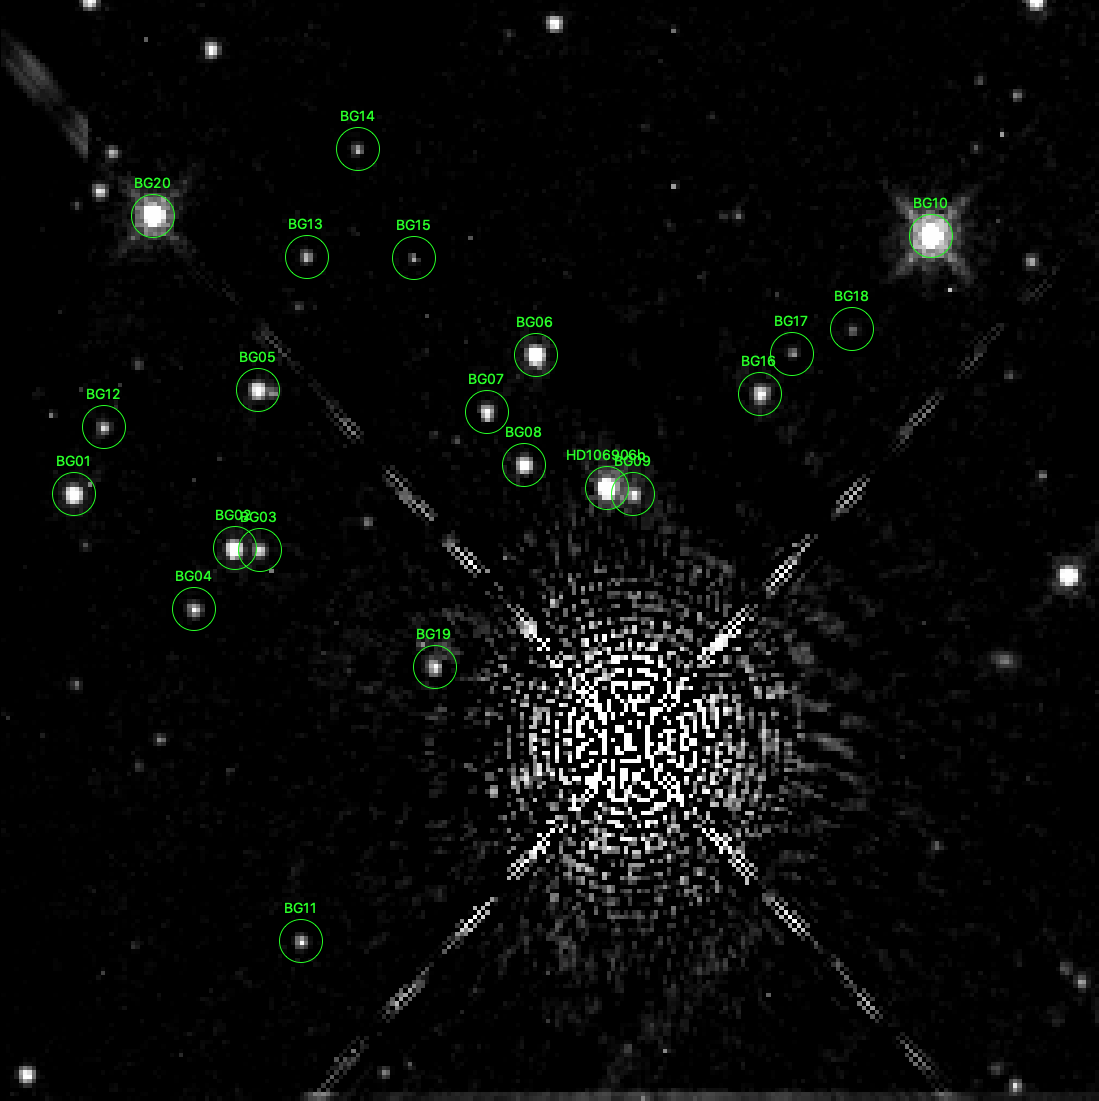
\includegraphics[width=0.5\textwidth]{figures/backSourceLabeled.png}
  \caption{Illustration of sky locations of background sources in the FoV.}
  \label{fig:bck}
\end{figure}


\begin{deluxetable*}{cccccc}
  
  \tablecaption{Background Sources in the Field of View\label{tab:bck}}
  
  \tablehead{
    \colhead{Source ID} &
    \colhead{RA (epoch 2016)} &
    \colhead{Dec (epoch 2016)} &
    \colhead{Flux$_{\mathrm{F127M}}$} &
    \colhead{Flux$_{\mathrm{F139M}}$} &
    \colhead{Flux$_{\mathrm{F153M}}$} \\
    \colhead{} &
    \colhead{hh mm ss} &
    \colhead{dd mm ss} &
    \colhead{\fluxunit} &
    \colhead{\fluxunit} &
    \colhead{\fluxunit} 
  }
  
  \startdata
BG01 & 12 17 53.4888 & -55 58 13.6500 & 1.91e-17 & 1.68e-17 & 1.49e-17 \\
BG02 & 12 17 53.3336 & -55 58 18.7430 & 1.76e-17 & 1.58e-17 & 1.33e-17 \\
BG03 & 12 17 53.2894 & -55 58 19.4400 & 3.43e-18 & 3.22e-18 & 2.93e-18 \\
BG04 & 12 17 53.5828 & -55 58 18.5440 & 3.48e-18 & 3.25e-18 & 2.83e-18 \\
BG05 & 12 17 52.8349 & -55 58 17.0570 & 1.12e-17 & 9.91e-18 & 8.39e-18 \\
BG06 & 12 17 52.1945 & -55 58 23.9900 & 2.96e-17 & 2.62e-17 & 2.22e-17 \\
BG07 & 12 17 52.4532 & -55 58 23.5060 & 5.58e-18 & 4.93e-18 & 4.24e-18 \\
BG08 & 12 17 52.5344 & -55 58 25.2920 & 1.11e-17 & 9.68e-18 & 8.70e-18 \\
BG09 & 12 17 52.4036 & -55 58 28.6550 & 4.22e-18 & 3.35e-18 & 3.37e-18 \\
BG10 & 12 17 51.0839 & -55 58 32.8790 & 2.72e-16 & 2.44e-16 & 2.08e-16 \\
BG11 & 12 17 54.3210 & -55 58 26.2290 & 2.94e-18 & 2.61e-18 & 2.46e-18 \\
BG12 & 12 17 53.2405 & -55 58 13.4710 & 2.66e-18 & 2.39e-18 & 2.21e-18 \\
BG13 & 12 17 52.3609 & -55 58 16.4220 & 2.11e-18 & 1.84e-18 & 1.71e-18 \\
BG14 & 12 17 51.9528 & -55 58 16.2300 & 1.70e-18 & 1.53e-18 & 1.41e-18 \\
BG15 & 12 17 52.1558 & -55 58 19.3130 & 1.17e-18 & 1.05e-18 & 8.63e-19 \\
BG16 & 12 17 51.6896 & -55 58 30.8770 & 8.44e-18 & 7.23e-18 & 6.33e-18 \\
BG17 & 12 17 51.8690 & -55 58 30.5800 & 1.04e-18 & 1.04e-18 & 9.03e-19 \\
BG18 & 12 17 51.5059 & -55 58 32.1210 & 7.17e-19 & 6.32e-19 & 5.02e-19 \\
BG19 & 12 17 53.2804 & -55 58 25.8250 & 5.48e-18 & 4.02e-18 & 3.26e-18 \\
BG20 & 12 17 52.5365 & -55 58 11.7060 & 1.36e-16 & 1.20e-16 & 1.05e-16 
  \enddata
\end{deluxetable*}

\bibliographystyle{yahapj}
\bibliography{library}


\end{document}

%%% Local Variables:
%%% mode: latex
%%% TeX-master: t
%%% End:

% LocalWords:  AAS
